\documentclass{article}

\usepackage[T1]{fontenc}

\usepackage{graphicx}
\graphicspath{ {./obrazki/} }
\usepackage{wrapfig}
\usepackage[export]{adjustbox}
\usepackage{polski}
\usepackage[utf8]{inputenc}
\usepackage[polish]{babel}
\usepackage{gensymb}
\usepackage{xfrac}
\usepackage{anyfontsize}

\title{Pyszności}
\author{Kingi i Mateusza}
\date{2020-03-29}

\begin{document}
    \pagenumbering{gobble}
    \maketitle
    \newpage
    \tableofcontents
    \newpage
    \pagenumbering{arabic}

    % #########################################################################
    % #########################################################################
    % #########################################################################
    \section{Dania obiadowe}
    \medskip
    \subsection{Tortilla}
    \bigskip
    \paragraph{Składniki:}
    \begin{wrapfigure}[1]{r}{0.4\textwidth}
        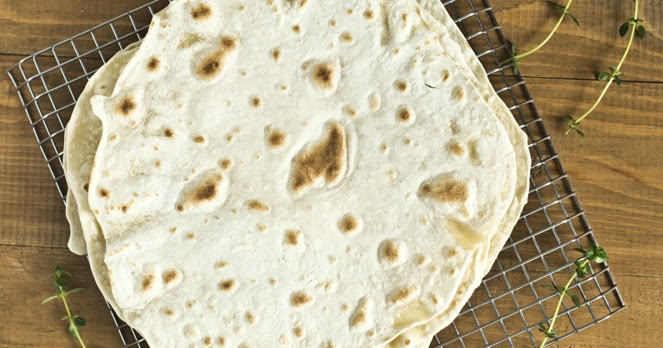
\includegraphics[width=0.4\textwidth]{tortilla.jpg}
    \end{wrapfigure}
    \begin{enumerate}
        \item 250g mąki (tortowa z Łasina)
        \item \sfrac{1}{2} szklanki gorącej wody
        \item \sfrac{1}{2} łyżeczki soli
        \item 2 łyżki smalcu
    \end{enumerate}

    \paragraph{Przygotowanie:}
    \begin{enumerate}
        \item Mąkę przesiewamy do miski.
        \item Smalec rozpuszczamy w gorącej wodzie z dodatkiem soli.
        \item Wyrabiamy ciasto przez około 10 minut.
        \item Ciasto dzielimy na około 8-10 części i rozwałkujemy na stolnicy,
            do przezroczystości.
        \item Smażymy placki tortilli na suchej, teflonowej lub ceramicznej
            patelni po ok. 2-4 minuty z każdej storny, aż do uzyskania
            brązowych, rumianych plamek.
        \item Gorące placki nadziewamy farszem i zawijamy.
    \end{enumerate}

    \paragraph{Porada}
    Zimne placki tracą swoją elastyczność, przed zawijaniem należy podgrzać je
    na gorącej, suchej patelni.
    \newpage


    \subsection{Pancakes}
    \bigskip
    \paragraph{Składniki:}
    \begin{wrapfigure}[1]{r}{0.4\textwidth}
        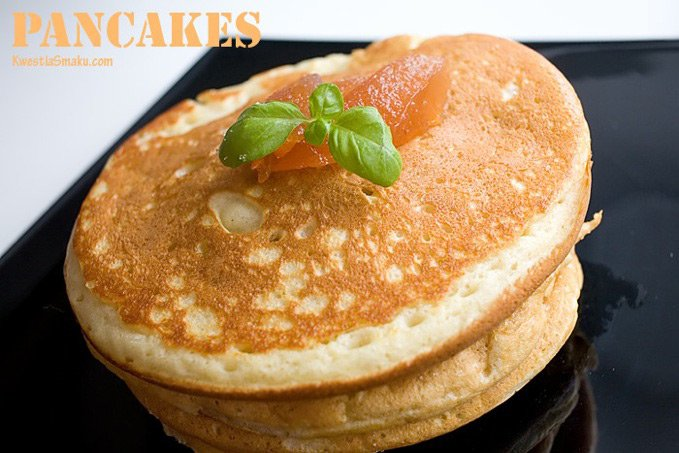
\includegraphics[width=0.4\textwidth]{pancakes.jpg}
    \end{wrapfigure}
    \begin{enumerate}
        \item 2 szklanki mąki
        \item 2 jajka
        \item $1\sfrac{1}{2}$ szklanki mleka
        \item 75 g rozpuszczonego masła
        \item $3\sfrac{1}{2}$ łyżeczki proszku do pieczenia
        \item \sfrac{1}{3} szklanki cukru pudru/cukru brązowego
        \item szczypta soli
    \end{enumerate}

    \paragraph{Przygotowanie}
    \begin{enumerate}
        \item Mąkę przesiać.
        \item Jajka roztrzepać i wymieszać z mlekiem, następnie połączyć z
            pozostałymi składnikami, na końcu dodać masło.
        \item Odstawić na 15 minut.
        \item Smażyć na suchej patelni teflonowej, bez dodatkowego tłuszczu, na
            średnim ogniu, tak aby dać ciastu szansę na wyrośnięcie.
        \item Delikatnie przewrócić na drugą stronę, przy użyciu szerokiej
            łopatki.
    \end{enumerate}
    \newpage


    \subsection{Naleśniki}
    \bigskip
    \paragraph{Składniki:}
    \begin{wrapfigure}[1]{r}{0.4\textwidth}
        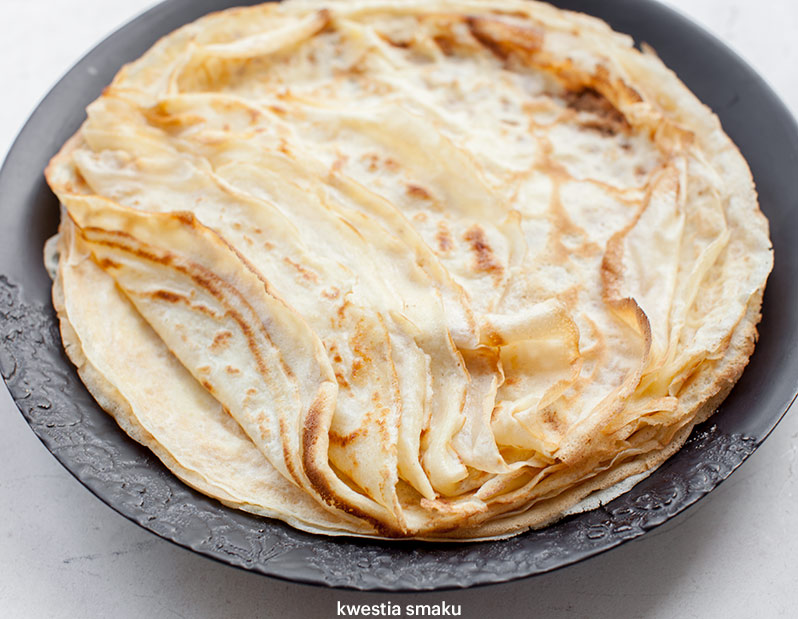
\includegraphics[width=0.4\textwidth]{nalesniki.jpg}
    \end{wrapfigure}
    \begin{enumerate}
        \item 1 szklanka mąki pszennej
        \item 2 jajka
        \item 1 szklanka mleka
        \item \sfrac{3}{4} szklanki wody (najlepiej gazowanej)
        \item szczypta soli
        \item 3 łyżki masła lub oleju roślinnego
    \end{enumerate}

    \paragraph{Przygotowanie:}
    \begin{enumerate}
        \item Mąkę wsypać do miski, dodać jajka, mleko, wodę i sól. Zmiksować na
            gładkie ciasto.
        \item Dodać roztopione masło lub olej roślinny i razem zmiksować (lub
            wykorzystać tłuszcz do smarowania patelni przed smażeniem każdego
            naleśnika).
        \item Naleśniki smażyć na dobrze rozgrzanej patelni z cienkim dnem np.
            naleśnikowej. Przewrócić na drugą stronę gdy spód naleśnika będzie
            już ładnie zrumieniony i ścięty.
    \end{enumerate}
    \newpage


    \subsection{Roladki nadziewane pesto z dodatkiem suszonych pomidorów}
    \bigskip
    \paragraph{Składniki:}
    \begin{wrapfigure}[1]{r}{0.4\textwidth}
        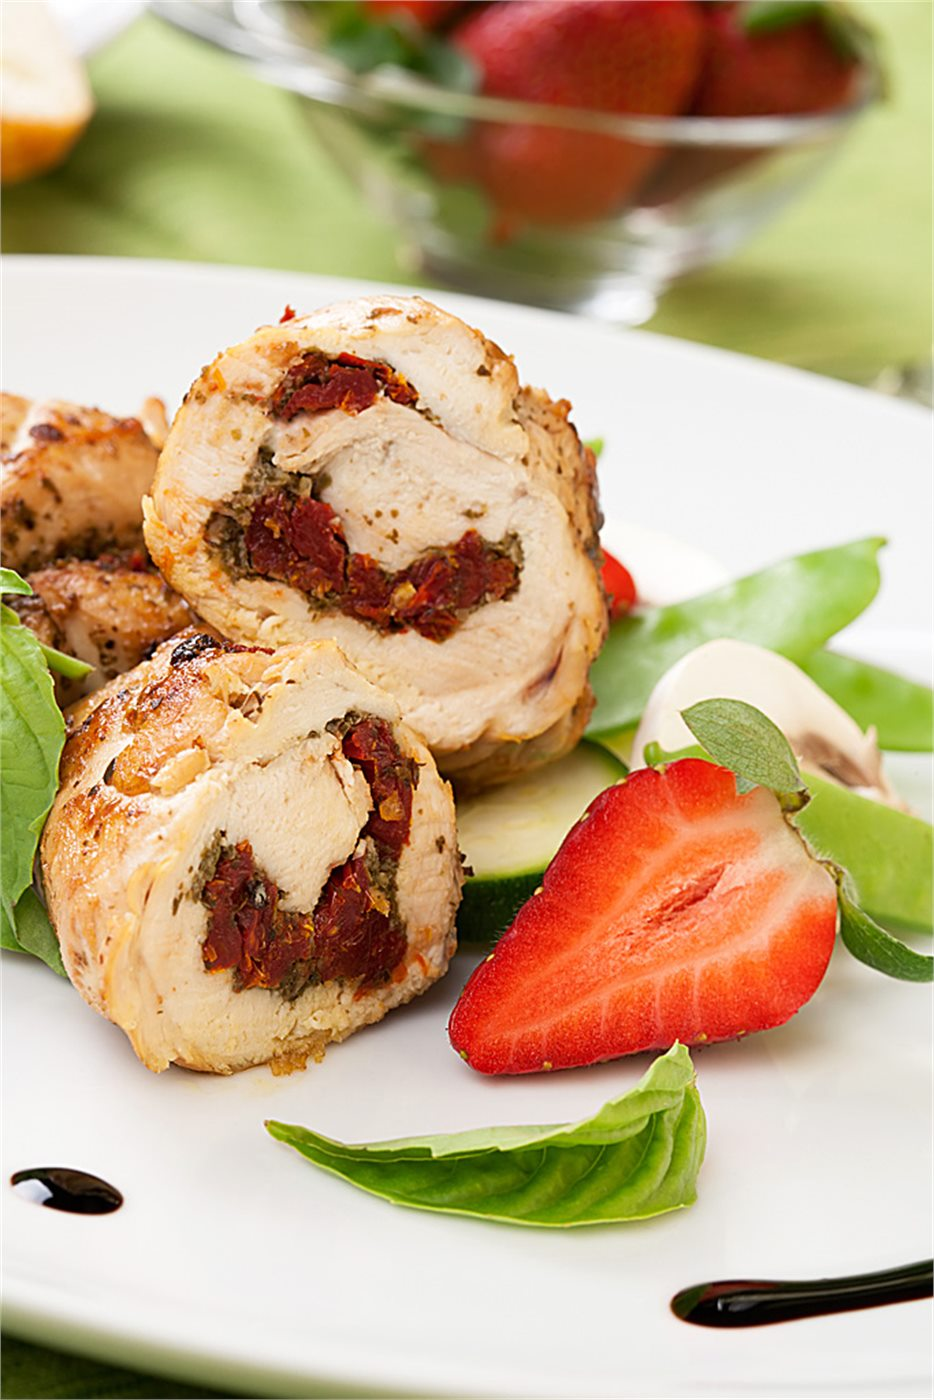
\includegraphics[width=0.4\textwidth, height=0.5\textwidth]{roladki-z-suszonymi-pomidorami-i-pesto.jpg}
    \end{wrapfigure}
    \begin{enumerate}
        \item Filet z piersi kurczaka - 2,25 porcji (230 g)
        \item Zielone pesto - 2 łyżeczki (35 g)
        \item Pomidory suszone na słońcu - 1,25 garści (35 g)
        \item Ryż brązowy - 0,75 szklanki (120 g)
        \item Pieczarki - 3,25 garści (190 g)
        \item Sól - 2 szczypty (1 g)
        \item Pieprz czarny ziarnisty - 2 szczypty (1 g)
        \item Chilli - 2 szczypty (1 g)
        \item Kurkuma - 2 szczypty (1 g)
    \end{enumerate}

    \paragraph{Przygotowanie}
    \begin{enumerate}
        \item Piersi z kurczaka rozbij tłuczkiem przez folię, tak by nie
            zostawić dziur, posmaruj pesto i dodaj przekrojone na pół plasterki
            suszonych pomidorów. Tak przygotowane mięso zawiń w roladki.
        \item Piekarnik nagrzej do $180\degree$C. W naczyniu żaroodpornym ułóż
            przygotowane roladki. Naczynia nie przykrywaj.
        \item Kiedy mięso delikatnie się zarumieni (po ok. 15–20 minutach)
            podlej je wodą i przykryj naczynie. Piecz mięso jeszcze ok. 10–15
            minut.
        \item W osobnym garnku z grubym dnem podduś na odrobinie wody pieczarki
            razem z przyprawami i dodaj do gotowego mięsa w formie sosu.
        \item Danie podawaj z osobno ugotowanym al dente brązowym ryżem.
    \end{enumerate}
    \newpage


    \subsection{Kebab}
    \bigskip
    \paragraph{Składniki:}
    \begin{wrapfigure}[1]{r}{0.4\textwidth}
        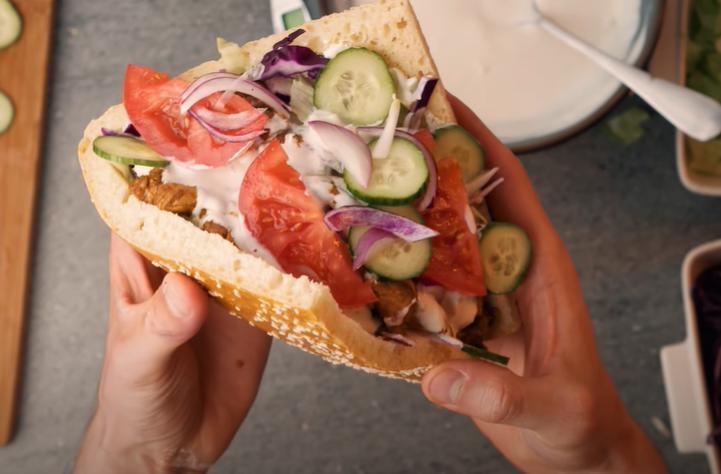
\includegraphics[width=0.4\textwidth]{kebab.jpg}
    \end{wrapfigure}
    \begin{enumerate}
        \item Bułka:
        \begin{enumerate}
            \item Mąka pszenna typ 650 – 400g
            \item Ciepła woda - 150ml
            \item Jogurt naturalny – 100g
            \item Sól – 10g
            \item Oliwa – 10ml
            \item Drożdże świeże – 25g $/$ suche ok 7-8g
            \item Żółtko jajka do posmarowania bułki
            \item Sezam do posypania
        \end{enumerate}
        \item Mięsko do kebaba:
        \begin{enumerate}
            \item Mięso z udka kurczaka – 500g
            \item Przyprawa do kurczaka –  1 płaska łyżka
            \item Oliwa – 5 ml
            \item Przyprawa Garam Masala – 1 płaska łyżka
        \end{enumerate}
        \item Sos czosnkowy:
        \begin{enumerate}
            \item Skyr – 150g
            \item Jogurt naturalny – 100g
            \item Majonez – 50 g
            \item Czosnek -1 lub 2 ząbki
        \end{enumerate}
        \item Dodatki:
        \begin{enumerate}
            \item Sałata lodowa $/$ pekinka
            \item Czerwona cebulka
            \item Ogórek
            \item Pomidor
        \end{enumerate}
    \end{enumerate}

    \paragraph{Przygotowanie:}
    \begin{enumerate}
    \item Dzień wcześniej:
    \begin{enumerate}
        \item Mięso wymieszać z marynatą i odstawić do lodówki na kilka godzin.
        \item Czosnek kroimy drobno i mieszamy z resztą składników. Odstawiamy
            do lodówki na kilka godzin, aby smaki się przegryzły.
    \end{enumerate}
    \item Przygotowanie:
    \begin{enumerate}
        \item Ciepłą wodę mieszamy z drożdżami i łyżką mąki aż do zlikwidowania
            grudek. Odstawiamy na 10 min.
        \item Po tym czasie mieszamy wszystkie składniki. Wyrabiamy ciasto ok
            10-15 min.
        \item Gotowe ciasto wkładamy do miski i przykrywamy folią spożywczą (aby
            cisto nie wyschło). Odstawiamy na 1 godzinę.
        \item Po tym czasie wałkujemy ciasto na okrąg o średnicy $28-30cm$.
            Wierzch ciasta polewamy rozbełtanym żółtkiem i posypujemy sezamem.
        \item Pieczemy w 200 stopniach, grzanie góra – dół, 25 min.
        \item Smażymy wcześniej zamarynowane mięso.
        \item Po wyciągnięciu z piekarnika i po wystygnięciu bułki, kroimy ją na
            4 części. Następnie kroimy ją wzdłuż.
    \end{enumerate}
    \end{enumerate}
    \newpage


    \subsection{Polędwiczki w sosie własnym}
    \bigskip
    \paragraph{Składniki:}
    \begin{wrapfigure}[1]{r}{0.4\textwidth}
        \includegraphics[width=0.4\textwidth]{poledwiczki_w_sosie_własnym.jpg}
    \end{wrapfigure}
    \begin{enumerate}
        \item 0,5 kg polędwiczek wieprzowych
        \item 1 cebula
        \item 1 ząbek czosnku
        \item 2 łyżki oleju
        \item 1 łyżka mąki pszennej
        \item 1 łyżeczka suszonego majeranku
        \item 0,5 łyżeczki słodkiej, mielonej papryki
        \item sól, pieprz do smaku
    \end{enumerate}

    \paragraph{Przygotowanie}
    \begin{enumerate}
        \item Umyte, osuszone i oczyszczone z włókien mięso kroję na plastry
            grubości ok. 1,5 cm, każdy oprószam lekko solą, pieprzem i mąką.
        \item Rozgrzewam olej na patelni i obsmażam mięso z obu stron, na
            rumiano (najlepiej podzielić mięso na dwie porcje).
        \item Usmażone mięso zdejmuję z patelni, a na nią wrzucam pokrojoną w
            kostkę cebule i smażę do zeszklenia na tym samym oleju.
        \item Z powrotem przekładam mięso, zalewam je wodą by je prawie pokryła,
            dodaję majeranek i paprykę i posiekany czosnek, lekko wszystko solę
            i oprószam pieprzem.
        \item Przykrywam i duszę na wolnym ogniu ok. 35-40 minut, aż mięso
            będzie miękkie.
    \end{enumerate}
    \newpage


    \subsection{Polędwiczki z indyka w sosie porowo-śmietanowym}
    \bigskip
    \paragraph{Składniki:}
    \begin{wrapfigure}[2]{r}{0.4\textwidth}
        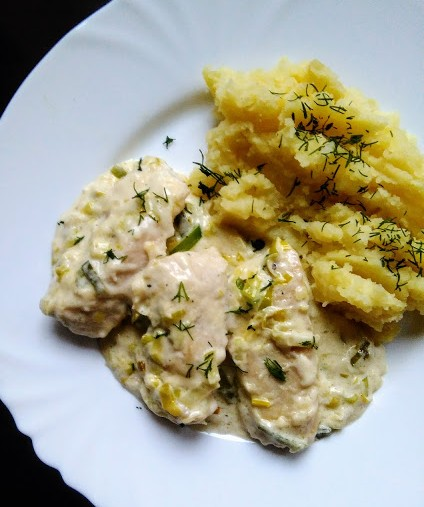
\includegraphics[width=0.4\textwidth]{poledwiczki_z_indyka_w_sosie_porowo_smietanowym.jpg}
    \end{wrapfigure}
    \begin{enumerate}
        \item 500 g polędwiczek z indyka (filet z piersi kurczaka, polędwiczki)
        \item sól i pieprz
        \item mąka do obtoczenia mięsa
        \item masło klarowane do smażenia
        \item 1 duży por lub 2 małe (biała i jasnozielona część)
        \item 300 ml śmietanki kremówki, min. 30\%
    \end{enumerate}

    \paragraph{Przygotowanie:}
    \begin{enumerate}
        \item Por oczyścić, dokładnie umyć i przekroić wzdłuż na pół, następnie
            pokroić w cienkie półplasterki.
        \item Mięso oczyścić z błonek i według własnego gustu pokroić na
            mniejsze części lub zostawić w całości. Ja polędwiczki z indyka
            pokroiłam w poprzek na plastry grubości około 2-3 cm. Mięso oprószyć
            solą i pieprzem z każdej strony i obtoczyć w mące.
        \item Na patelni z grubym dnem rozgrzać łyżkę masła klarowanego i na
            dość sporej mocy palnika podsmażyć mięso z każdej strony.
            Podsmażone mięso zdjąć z patelni i odłożyć na bok.
        \item Na patelni rozgrzać jeszcze łyżkę masła, dodać pokrojonego
            wcześniej pora, posolić, przesmażyć, następnie przykryć patelnię
            pokrywką i poddusić około 5 min aż por zmięknie.
        \item Następnie wlać śmietankę kremówkę i zagotować. Po zagotowaniu
            doprawić solą i pieprzem do smaku, do sosu włożyć usmażone wcześniej
            mięso, patelnię przykryć pokrywką i poddusić jeszcze około 10 min na
            małym ogniu aż mięso będzie miękkie.
        \item Podawać z ulubionymi dodatkami.
    \end{enumerate}
    \newpage


    \subsection{Szynka w sosie własnym}
    \bigskip
    \paragraph{Składniki}
    \begin{wrapfigure}[2]{r}{0.4\textwidth}
        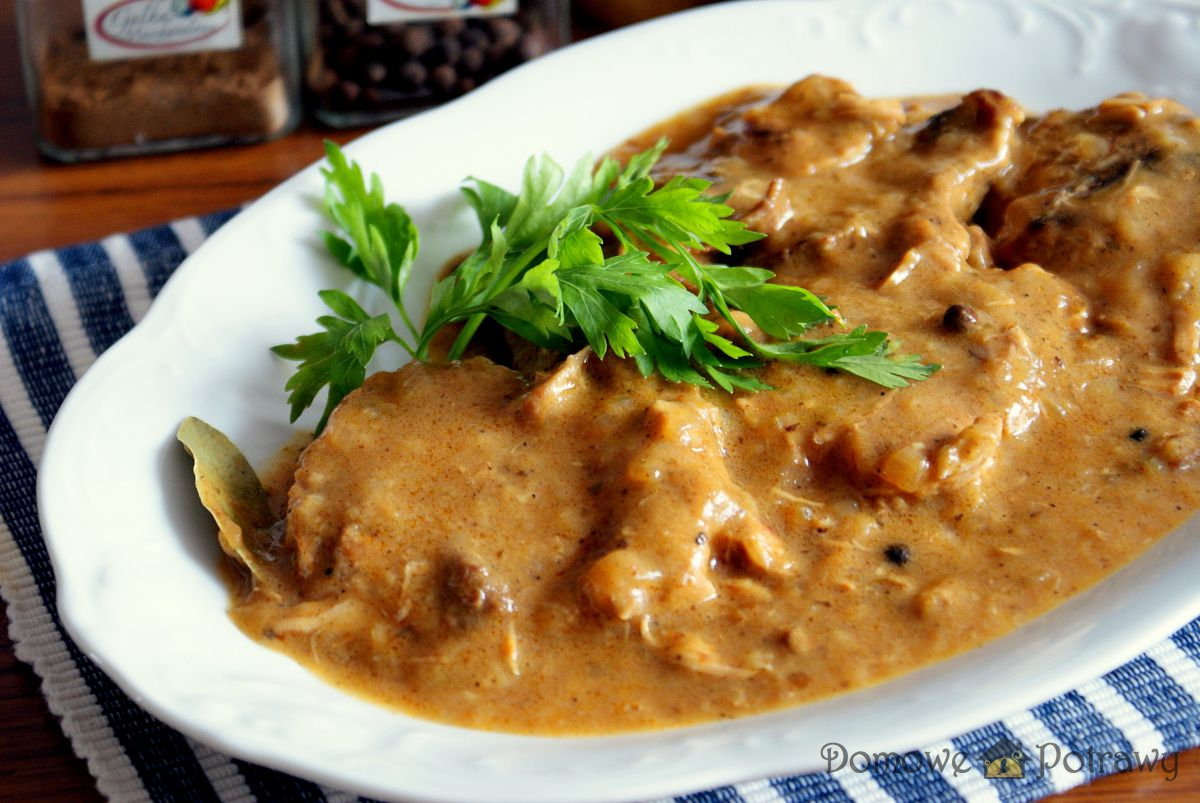
\includegraphics[width=0.4\textwidth]{szynka_w_sosie_wlasnym.jpg}
    \end{wrapfigure}
    \begin{enumerate}
    \item Sos
        \begin{enumerate}
            \item 1kg szynki wieprzowej bez kości
            \item 2 cebule
            \item bulion warzywny lub kostka mięsna
            \item 2 liście laurowe
            \item 3 ziarenka ziela angielskiego
            \item 4 ziarenka pieprzu
            \item 2-3 łyżki mąki
            \item 2 łyżki gęstej śmietany 18\%
        \end{enumerate}
     \item Marynata
        \begin{enumerate}
            \item 2 łyżki octu balsamicznego
            \item 4 łyżki oleju
            \item 1 łyżka ostrej musztardy (np. kozaka, dijon, sarepska)
            \item 1 łyżeczka miodu
            \item 2-3 łyżeczki majeranku
            \item 1 łyżeczka mielonej słodkiej papryki
            \item \sfrac{1}{3} łyżeczki ostrej papryki
            \item \sfrac{1}{2} łyżeczki mielonej gałki muszkatołowej
            \item 2 ząbki czosnku
            \item 1 płaska łyżeczka soli, pieprz
        \end{enumerate}
    \end{enumerate}

    \paragraph{Przygotowanie:}
    \begin{enumerate}
        \item Mięso z szynki umyć pod bieżącą wodą, osuszyć papierowym
            ręcznikiem i pokroić na plastry o grubości około 1,5 cm. Rozbić
            tłuczkiem. Oprószyć solą i pieprzem.
        \item Marynata do mięsa: W miseczce przygotować marynatę. Wszystkie jej
            składniki połączyć. Każdy plaster mięsa smarować marynatą i układać
            jeden na drugim w misce. Przykryć folią spożywczą i wstawić do
            lodówki przynajmniej na 1 godzinę lub dłużej, jeśli dysponujemy
            większą ilością czasu.
        \item Cebule pokroić kostkę i zeszklić na patelni. Następnie przełożyć
            do dużego rondla. Na tym samym tłuszczu podsmażyć na dużym ogniu
            mięso partiami, aby wyraźnie się zarumieniło. Przełożyć do rondla.
            Dodać liście laurowe, ziele angielskie oraz pieprz. Zalać taką
            ilością wody/bulionu, by ledwie przykrywała mięso. Dusić na małym
            ogniu przez około 1,5 godziny, aż mięso będzie wyraźnie kruche i
            miękkie. W razie potrzeby podczas duszenia dolać trochę wody.
        \item W kubeczku, w niewielkiej ilości zimnej wody rozrobić mąkę, dodać
            nieco wywaru z mięsa i śmietanę. Dodać do mięsa i dokładnie
            wymieszać.  Doprowadzić do zagotowania. Na koniec w razie potrzeby
            doprawić danie solą i pieprzem. Szynkę w sosie własnym podawać z
            ziemniakami purée, ryżem, bądź dowolną kaszą oraz surówką. Dobrze
            pasują tutaj np. buraczki na zimno, surówka z pora albo surówka z
            białej kapusty.
    \end{enumerate}
    \newpage


    \subsection{Zupa dyniowa}
    \bigskip
    \paragraph{Składniki:}
    \begin{wrapfigure}[1]{r}{0.4\textwidth}
        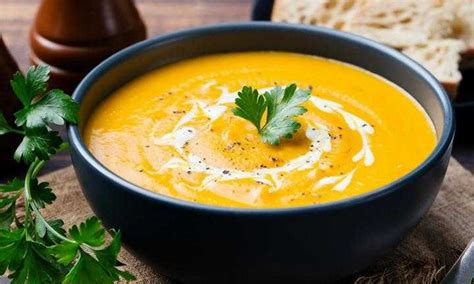
\includegraphics[width=0.4\textwidth]{zupa_dyniowa.jpg}
    \end{wrapfigure}
    \begin{enumerate}
        \item Dynia
        \item Rosół
        \item Cebula
        \item Czosnek
        \item 4 Ziemniaki
        \item Imbir
        \item Gałka muszkatałowa
    \end{enumerate}

    \paragraph{Przygotowanie}
    \begin{enumerate}
        \item Z rosołu wyciągnąć mięso, i warzywa które nie mają zostać zblendowane.
        \item W rosole ugotować ziemniaki. Na patelni podsmażyć cebulę, czosnek i dynię.
        \item Przygotować grzanki - chleb pokroić w kostkę, doprawić przyprawami.
        \item Gdy dynia zmięknie dodać ją do rosołu z ziemniakami. Zblendować zawartość garnka.
        \item Doprawić imbirem, gałką muszkatałową i w razie potrzeby solą i pieprzem.
    \end{enumerate}
    \newpage


    \subsection{Kluski ziemniaczane}
    \bigskip
    \paragraph{Składniki:}
    \begin{wrapfigure}[1]{r}{0.4\textwidth}
        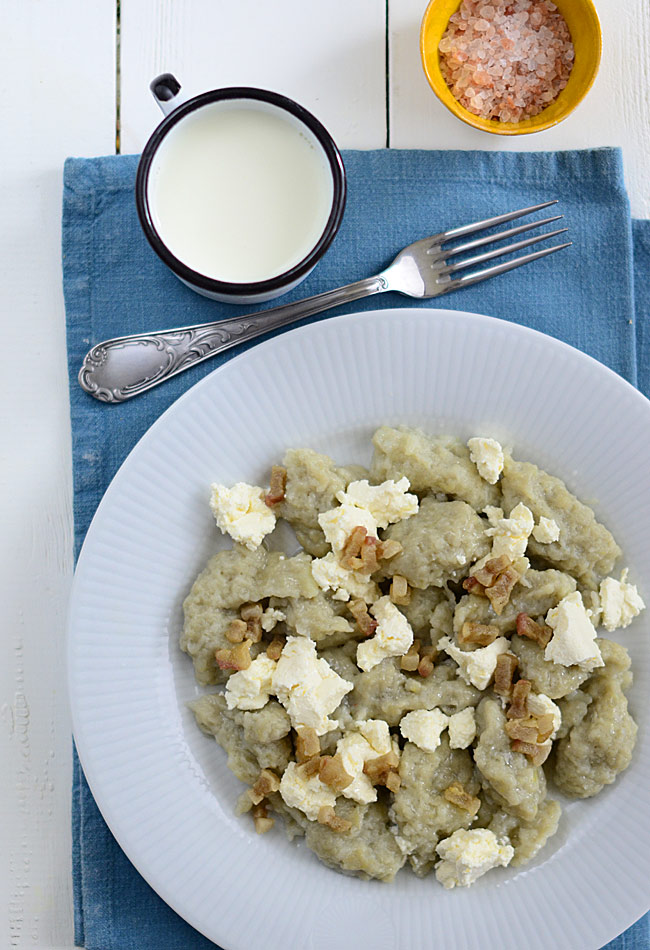
\includegraphics[width=0.4\textwidth, height=0.5\textwidth]{kluski_ziemniaczane.jpg}
    \end{wrapfigure}
    \begin{enumerate}
        \item 1\sfrac{1}{2} kg ziemniaków
        \item mąką (około 14 bardzo czubatych łyżek)
        \item 1 jajko
        \item sól
        \item 20 dkg chudej kiełbasy lub boczku
        \item 1 średnia cebulka
        \item 1 łyżka oleju
    \end{enumerate}

    \paragraph{Przygotowanie:}
    \begin{enumerate}
        \item Obrane ziemniaki,umyć,zetrzeć na tarce,tak jak na placki,wylać na
            sito lub durszlak ,pod spód podstawiając czysty garnek.
        \item Gdy woda z ziemniaków dobrze odleci,zlać delikatnie płyn, krochmal
            który został na dnie garnka,zebrać łyżką i włożyć do ziemniaków.
        \item Dodać 1 jajko,mąkę,i wymieszać,ciasto ma być gęste i lekko odstawać od łyżki.
        \item Wstawić wodę, posolić,wlać łyżeczkę oleju ,gdy woda się
            gotuje,maczamy łyżkę we wrzątku,i kładziemy łyżką kluseczki(wielkość
            dowolna) jak się będą lekko rozpadać, dodać jeszcze troszkę mąki.
        \item Gotować około 8 min od wypłynięcia.
        \item Boczek lub kiełbaskę, przesmażyć na łyżce oleju, razem z pokrojoną
            w kosteczkę cebulką,polać kluseczki.
    \end{enumerate}
    \newpage


    \subsection{Placki ziemniaczane}
    \bigskip
    \paragraph{Składniki:}
    \begin{wrapfigure}[1]{r}{0.4\textwidth}
        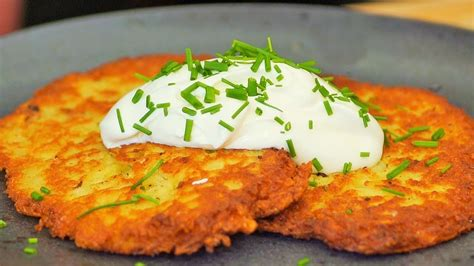
\includegraphics[width=0.4\textwidth]{placki_ziemniaczane.jpg}
    \end{wrapfigure}
    \begin{enumerate}
        \item 1 kg ziemniaków
        \item 6 łyżek mąki pszennej
        \item 1 jajko (opcjonalnie)
        \item 2 cebule
        \item olej do smażenia
        \item 2 kubki gęstej kwaśnej śmietany lub jogurtu naturalnego sojowego lub zwierzęcego
        \item sól i cukier do smaku
    \end{enumerate}

    \paragraph{Przygotowanie:}
    \begin{enumerate}
        \item Ziemniaki obrać, umyć pod bieżącą wodą i zetrzeć na tarce o
            drobnych oczkach. Odcisnąć dokładnie płyn, który należy zebrać do
            miseczki. Na dnie osadzi się skrobia, którą dodajemy do startych
            ziemniaków.
        \item Cebule obrać i zetrzeć na tarce o grubych oczkach.
        \item Ziemniaki wymieszać z jajkiem, mąką, startą cebulą, doprawić do
            smaku solą i smażyć partiami na gorącym tłuszczu.
        \item Placki ziemniaczane podawać ze śmietaną, cukrem lub solą.
    \end{enumerate}
    \newpage

%    \subsection{Naleśniki}
%    \bigskip
%    \paragraph{Składniki:}
%    \begin{wrapfigure}[1]{r}{0.4\textwidth}
%        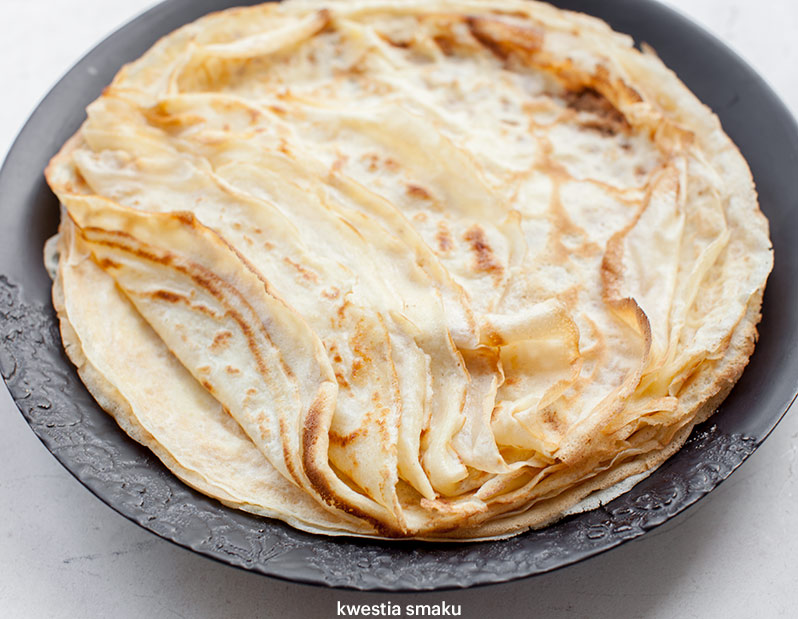
\includegraphics[width=0.4\textwidth]{nalesniki.jpg}
%    \end{wrapfigure}
%    \begin{enumerate}
%    \end{enumerate}
%
%    \paragraph{Przygotowanie}
%    \begin{enumerate}
%    \end{enumerate}
%    \newpage

    % #######################################################################
    % #######################################################################
    % #######################################################################
    \section{Desery}
    \medskip
    \subsection{Murzynek}
    \bigskip

    \paragraph{Składniki:}
    \begin{wrapfigure}[3]{r}{0.4\textwidth}
        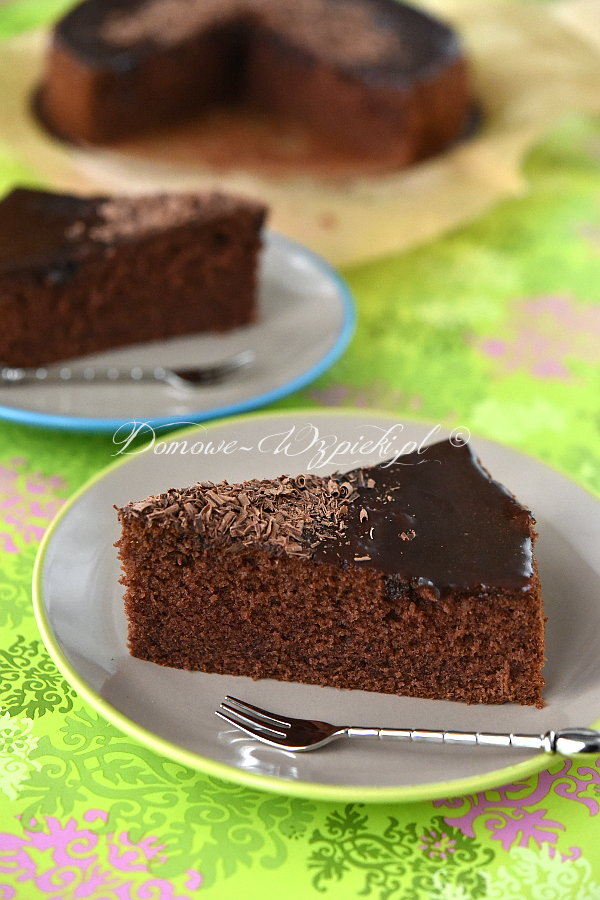
\includegraphics[width=0.4\textwidth, height=0.5\textwidth]{murzynek.jpg}
    \end{wrapfigure}
    \begin{enumerate}
        \item \sfrac{1}{2} szklanki mleka lub wody (125ml)
        \item 3 kopiate łyżki kakao
        \item 1\sfrac{1}{2} szklanki cukru (300g)
        \item 250g masła lub margaryny
        \item 4 jajka
        \item 1\sfrac{1}{2} szklanki mąki pszennej (225g)
        \item 2 łyżeczki proszku do pieczenia
    \end{enumerate}

    \paragraph{Przygotowanie}
    \begin{enumerate}
        \item Mleko, kakao i cukier przełożyć do garnka i mieszając, zagotować.
            Do gorącej masy dodać masło i mieszać, aż się rozpuści.  Pozostawić
            do ostygnięcia.
        \item Mąkę wymieszać z proszkiem do pieczenia, odstawić na bok.
        \item Jajka sparzyć wrzątkiem, oddzielić żółtka od białek. Białka ubić
            na sztyw-ną pianę, odstawić na bok. Żółtka wmieszać do ostygniętej
            masy. Odlać pół szklanki masy. Ostawić na bok. Wmieszać mąkę z
            proszkiem. Na końcu wmieszać delikatnie pianę z białek.
        \item Dno tortownicy o średnicy 26cm wyłożyć papierem do pieczenia, a
            następnie zacisnąć obręcz. Ciasto przełożyć do formy.
        \item Piec w nagrzanym piekarniku ok. 45 minut, do suchego patyczka, w
            temperaturze 180°C. Pozostawić do ostygnięcia.
        \item Ciasto polać odłożoną polewą. (Gdyby polewa była za rzadka, należy
            włożyć ją na chwilę do lodówki, aż lekko zgęstnieje).
    \end{enumerate}
    \newpage


    \subsection{Sernik królewski}
    \bigskip
    \paragraph{Składniki:}
    \begin{wrapfigure}[2]{r}{0.4\textwidth}
        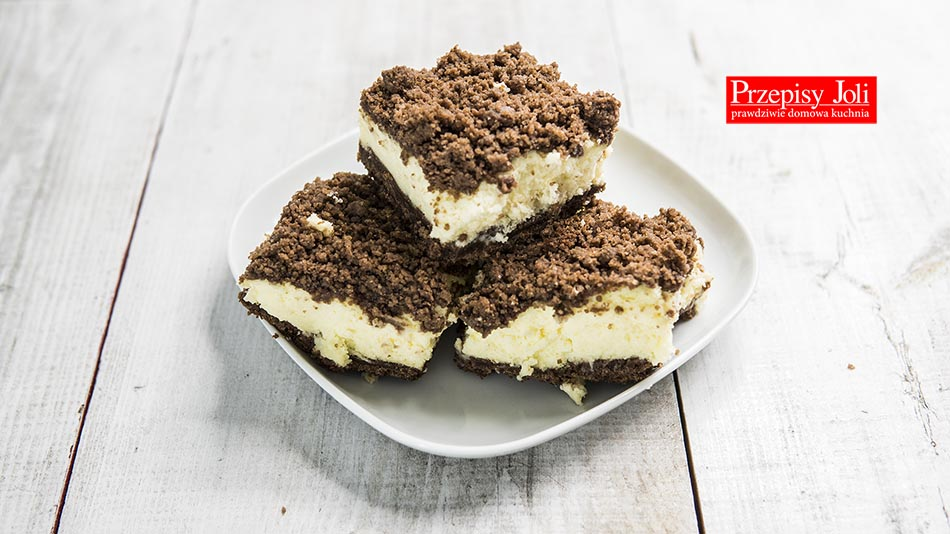
\includegraphics[width=0.4\textwidth]{sernik_krolewski.jpg}
    \end{wrapfigure}
    \begin{enumerate}
        \item Warstwa ciasta:
        \begin{enumerate}
            \item 3 szklanki mąki
            \item 1,5 szklanki cukru
            \item 1 łyżka cukru waniliowego
            \item 2 łyżki kakao
            \item 2 łyżeczki proszku do pieczenia
            \item 3 żółtka
            \item 300 g masła
        \end{enumerate}
        \item Warstwa sera:
        \begin{enumerate}
            \item 1 kg zmielonego białego sera
            \item 4 żółtka
            \item 1 szklanka cukru
            \item 200 g masła
            \item 2 budynie śmietankowe (bez cukru)
            \item 7 białek
        \end{enumerate}
    \end{enumerate}

    \paragraph{Przygotowanie:}
    \begin{enumerate}
        \item Do miski wsypujemy mąkę, cukier, cukier waniliowy, kakao, proszek
            do pieczenia, żółtka, i masło. Zagniatamy kruche ciasto (w tych
            proporcjach przypomina kruszonkę).
        \item Blaszkę o wymiarach 23x33 cm wykładamy papierem do pieczenia.
            Ciasto dzielimy na pół. Pierwszą połowę przekładamy na blaszkę i
            ubijamy.  Ciasto pieczemy przez 20 minut w temperaturze 180 stopni
            (góra-dół).
        \item W tym czasie przygotowujemy warstwę serową. Do misy miksera
            wlewamy białka, delikatnie solimy i ubijamy pianę. Pianę odkładamy
            na bok.
        \item Do misy miksera wrzucamy masło, żółtka, cukier i miksujemy na
            średnich obrotach. Następnie dodajemy ser (łyżka po łyżce) cały czas
            miksując.  Wsypujemy budyń i miksujemy do połączenia składników.
        \item Masę serową delikatnie mieszamy z ubitymi białkami (aż do
            połączenia).
        \item Po upieczeniu pierwszej warstwy wykładamy na nią masę serową. Na
            masę serową wykładamy warstwę ciasta.
        \item Ciasto pieczemy przez 40 minut w temperaturze 180 stopni (pieczeni
            góra-dół). Po upieczeniu studzimy w uchylonym piekarniku (żeby
            sernik mniej opadł).
    \end{enumerate}
    \newpage


    \subsection{Kruche ciastka z marmoladą}
    \bigskip

    \paragraph{Składniki:}
    \begin{wrapfigure}[3]{r}{0.4\textwidth}
        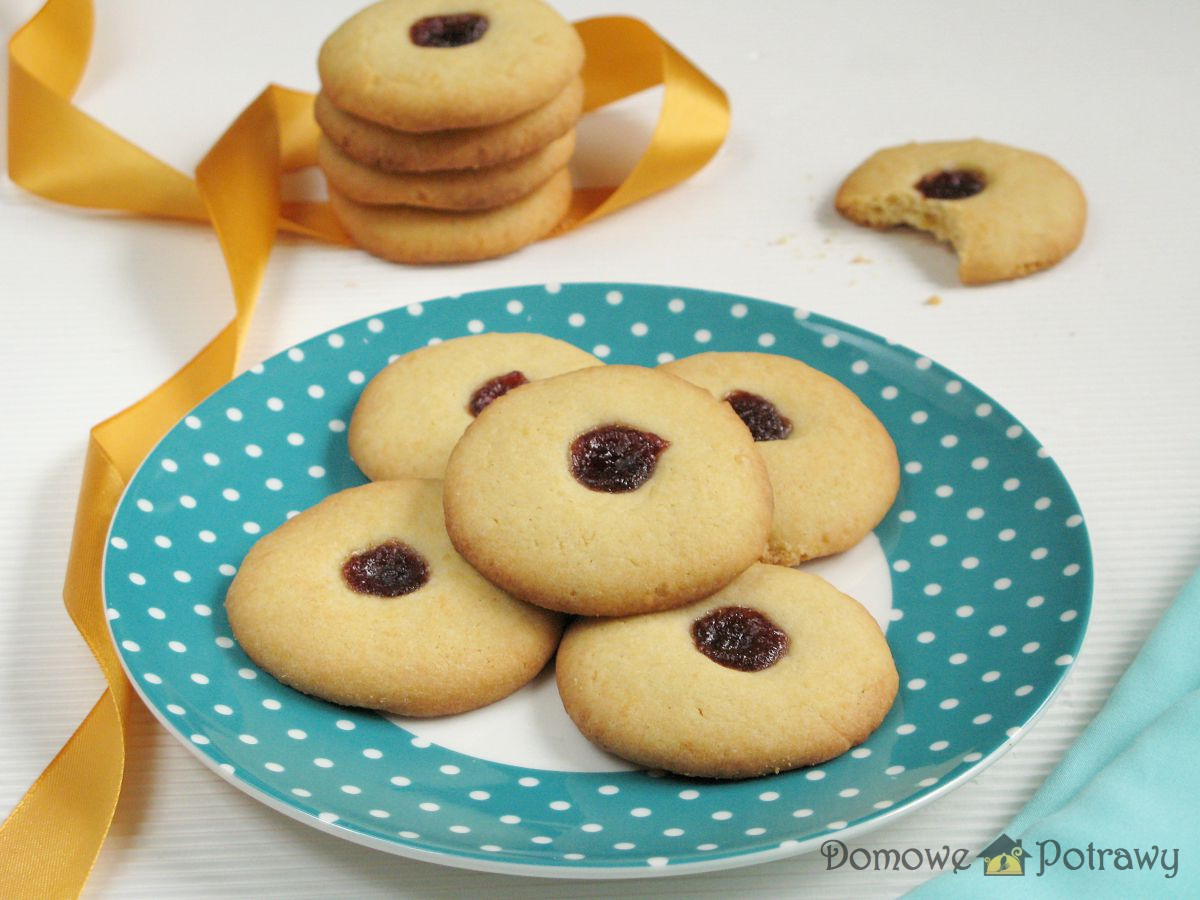
\includegraphics[width=0.4\textwidth]{kruche_ciasteczka_marmolada.jpg}
    \end{wrapfigure}
    \begin{enumerate}
        \item 3 szklanki mąki pszennej
        \item 250 zimnego masła lub margaryny
        \item 2 łyżki smalcu - zamiast smalcu można dać ewentualnie gęstą
            śmietanę 18\%
        \item 3 żółtka
        \item \sfrac{2}{3} szklanki cukru pudru
        \item 1 opakowanie cukru waniliowego (16g)
        \item 2 łyżeczki proszku do pieczenia
        \item szczypta soli
        \item dodatkowo: kilka łyżek marmolady
    \end{enumerate}

    \paragraph{Przygotowanie:}
    \begin{enumerate}
        \item Mąkę przesiać przez sito i wsypać do dużej miski. Zimne masło lub
            margarynę pokroić na nieduże kawałki. Wbić żółtka, dodać cukier
            puder, cukier waniliowy, proszek do pieczenia, masło bądź margarynę,
            smalec oraz szczyptę soli. Zagnieść elastyczne ciasto. Podsypać
            mąką, aby się nie kleiło.
        \item Ciasto owinąć w folię spożywczą lub aluminiową i wstawić do
            lodówki na 1 godzinę lub zamrażalnika na 30 minut. Ze schłodzonego
            ciasta odrywać małe kawałeczki wielkości orzecha włoskiego. Formować
            w dłoniach kulki, po czym je spłaszczać. Kłaść na wyłożonej papierem
            do pieczenia blaszce. W każdym ciastku zrobić palcem dziurkę.
        \item Kilka łyżek marmolady przełożyć do woreczka foliowego. Uciąć jeden
            z rogów. Wyciskać odrobinę marmolady do dziurki w ciastkach.
            Ciasteczka piec 15-20 minut w temperaturze $190\degree$C (wcześniej
            nagrzać piekarnik) do lekkiego zarumienia. Studzić na kratce.
            Ciasteczka przechowywać w zamkniętym pojemniku. Zachowują świeżość
            przez
            tydzień.
    \end{enumerate}
    \newpage


    \subsection{Bezy}
    \bigskip
    \paragraph{Składniki:}
    \begin{wrapfigure}[1]{r}{0.4\textwidth}
        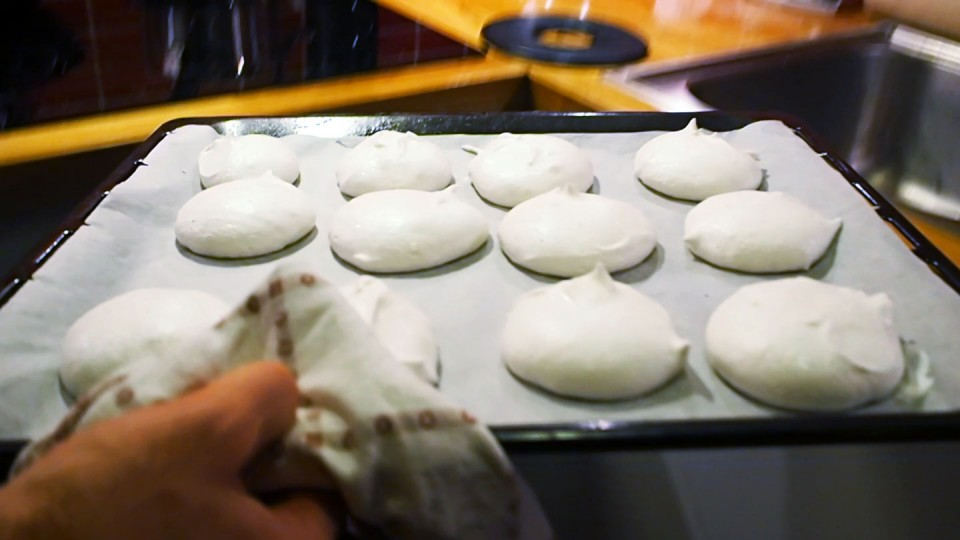
\includegraphics[width=0.4\textwidth]{bezy.jpg}
    \end{wrapfigure}
    \begin{enumerate}
        \item 60g cukru
        \item 60g cukru pudru
        \item białka z 2-3 jajek
        \item szczypta soli
    \end{enumerate}

    \paragraph{Przygotowanie:}
    \begin{enumerate}
        \item Wsypać 60g cukru i szczyptę soli do plastikowej miski.
        \item Dodać białka.
        \item Ubić na gęstą, sztywną pianę.
        \item Wmieszać cukier puder do ubitej piany.
        \item Wstawić do piekarnika nagrzanego do $100\degree$C, na
            45min-1h30min w zależności od preferencji i wielkości bez.
    \end{enumerate}
    \newpage


    \subsection{Gofry}
    \bigskip
    \paragraph{Składniki:}
    \begin{wrapfigure}[1]{r}{0.4\textwidth}
        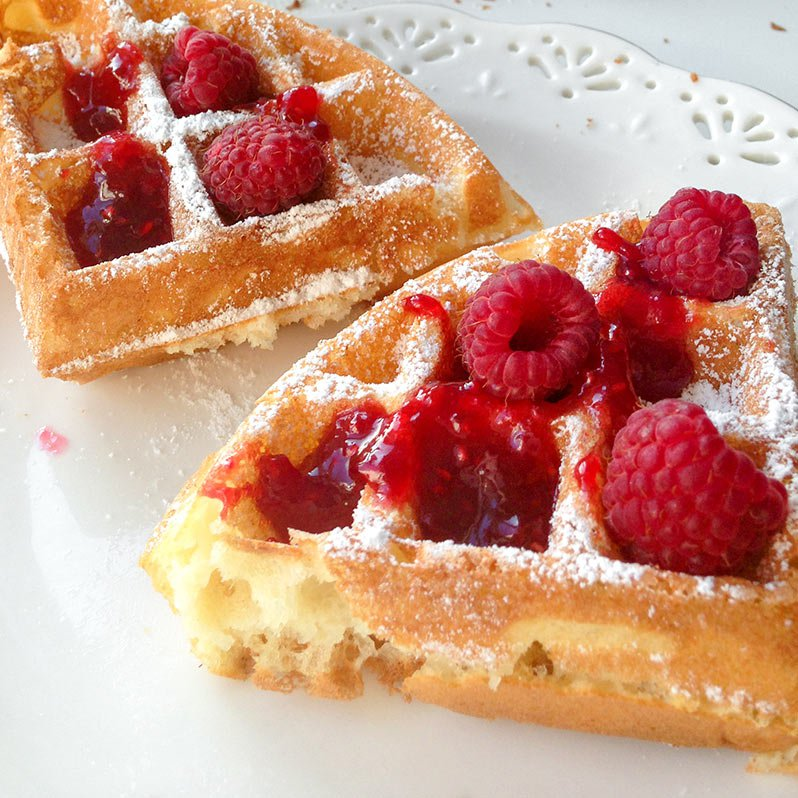
\includegraphics[width=0.4\textwidth]{gofry.jpg}
    \end{wrapfigure}
    \begin{enumerate}
        \item $1\sfrac{1}{2}$ szklanki mąki pszennej
        \item $1\sfrac{1}{2}$ łyżeczki proszku do pieczenia
        \item szczypta soli
        \item 2 łyżeczki cukru pudru lub kryształu
        \item 2 łyżeczki cukru wanilinowego
        \item 2 jaja
        \item \sfrac{1}{2} szklanki oleju roślinnego lub masła
        \item $1\sfrac{1}{3}$ szklanki mleka
    \end{enumerate}

    \paragraph{Przygotowanie:}
    \begin{enumerate}
        \item Mąkę wsypać do miski, dodać proszek do pieczenia, sól, cukier,
            cukier wanilinowy. Wszystko wymieszać a następnie dodać jajka, olej
            roślinny oraz mleko. Zmiksować mikserem na gładką masę, tylko do
            połączenia się składników. Ciasto można odstawić aby odpoczęło (na
            około 15 minut), ale nie jest to konieczne.
        \item Rozgrzać gofrownicę. Gofry piec przez około 3 - 3,5 minuty lub
            przez czas podany w instrukcji gofrownicy. Nakładamy ciasto chochlą
            i wypukłą stroną łyżki rozprowadzamy ciasto dokładnie po całej
            powierzchni.
        \item Gofry po upieczeniu odkładać na metalową kratkę. Posypać cukrem
            pudrem i polać syropem klonowym. Lub podawać z ulubionymi dodatkami
            np. marmoladą, dżemem, owocami i bitą śmietaną.
    \end{enumerate}
    \newpage


    \subsection{Biszkopt z musem}
    \bigskip
    \paragraph{Składniki:}
    \begin{wrapfigure}[2]{r}{0.4\textwidth}
        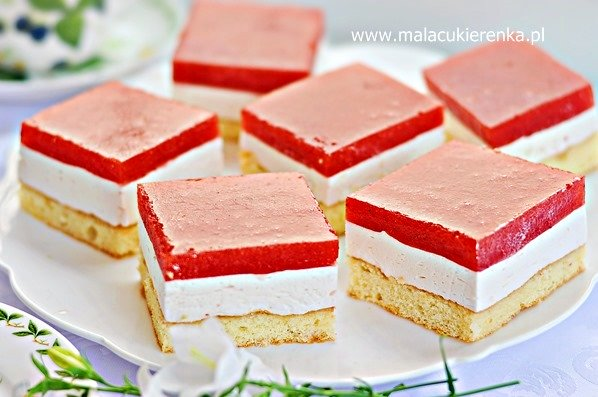
\includegraphics[width=0.4\textwidth]{biszkopt_z_musem.jpg}
    \end{wrapfigure}
    \begin{enumerate}
        \item Biszkopt:
        \begin{enumerate}
            \item 4 duże jajka – osobno żółtka i białka
            \item 100g cukru
            \item 140g mąki pszennej (użyłam tortowej)
            \item 1 płaska łyżeczka proszku do pieczenia
            \item \sfrac{1}{4} łyżeczki aromatu waniliowego
        \end{enumerate}
        \item Krem:
        \begin{enumerate}
            \item 1 galaretka truskawkowa w proszku
            \item 500g śmietanki kremówki 36\%
            \item 1 opakowanie cukru z prawdziwą wanilią lub cukier wanilinowy
                16g (można też dodać 1 łyżeczkę pasty waniliowej)
        \end{enumerate}
        \item Mus truskawkowy:
        \begin{enumerate}
            \item 2 galaretki truskawkowe w proszku lub czerwone w innym smaku
            \item 600g umytych, obranych truskawek
        \end{enumerate}
        \item Do nasączenia:
        \begin{enumerate}
            \item \sfrac{1}{3} szklanki wody
            \item 3 łyżki soku z cytryny
        \end{enumerate}
    \end{enumerate}

    \paragraph{Przygotowanie:}
    \paragraph{Biszkopt}
    \begin{enumerate}
        \item Mąkę przesiać i wymieszać z proszkiem do pieczenia.
        \item Piekarnik nastawić na $160\celsius$ na funkcji termoobieg (na funkcji
            góra-dół $170\celsius$).
        \item Białka ubić na sztywną pianę. Ciągle ucierając mikserem, stopniowo
            dodawać cukier, mieszać, aż masa stanie się gęsta i lśniąca.
        \item Następnie do białek dodać żółtka i jeszcze przez chwilę ucierać
            mikserem, aż powstanie kremowa, jednolita masa. Dodać aromat,
            wymieszać.
        \item Do jajecznej masy dodać w dwóch partiach wcześniej przygotowaną
            mąkę i po każdym dodaniu wymieszać delikatnie łyżką. Ciasto
            przełożyć do blaszki o wymiarach 25x35cm wyłożonej papierem do
            pieczenia, tylko dno. Wyrównać i wstawić do nagrzanego piekarnika.
            Piec przez około 40 minut.
        \item Po wyjęciu z piekarnika odstawić do całkowitego
            ostygnięcia.
        \item Biszkopt wyjąć z blaszki i zdjąć ostrożnie papier.  Następnie
            papier i biszkopt włożyć z powrotem do blaszki (dzięki temu ciasto
            będzie się lepiej kroiło).
        \item Składniki do nasączenia wymieszać i gotowym ponczem nasączyć
            biszkopt w blaszce.
    \end{enumerate}
    \paragraph{Krem}
    \begin{enumerate}
        \item Truskawkową galaretkę rozpuścić w 200ml gorącej wody, odstawić do
            całkowitego ostygnięcia.
        \item Śmietankę kremówkę ubić na sztywno z cukrem pudrem i cukrem z
            wanilią. Następnie cały czas mieszając mikserem, wlewać powoli lekko
            tężejącą galaretkę, dokładnie wymieszać.
        \item Gotowy krem wyłożyć na biszkopt, wyrównać. Blaszkę wstawić do
            lodówki.
    \end{enumerate}
    \paragraph{Mus truskawkowy}
    \begin{enumerate}
        \item Dwie galaretki rozpuścić w 500ml gorącej wody i odstawiać do
            całkowitego ostygnięcia.
        \item Truskawki zmiksować na mus, dodać ostygniętą galaretkę, wymieszać.
        \item Mus truskawkowy wylać na ciasto w blaszce i znów ciasto wstawić do
            lodówki na parę godzin, aż mus stężeje.
    \end{enumerate}
    \newpage


    \subsection{Muffiny z truskawkami}
    \bigskip
    \paragraph{Składniki:}
    \begin{wrapfigure}[2]{r}{0.4\textwidth}
        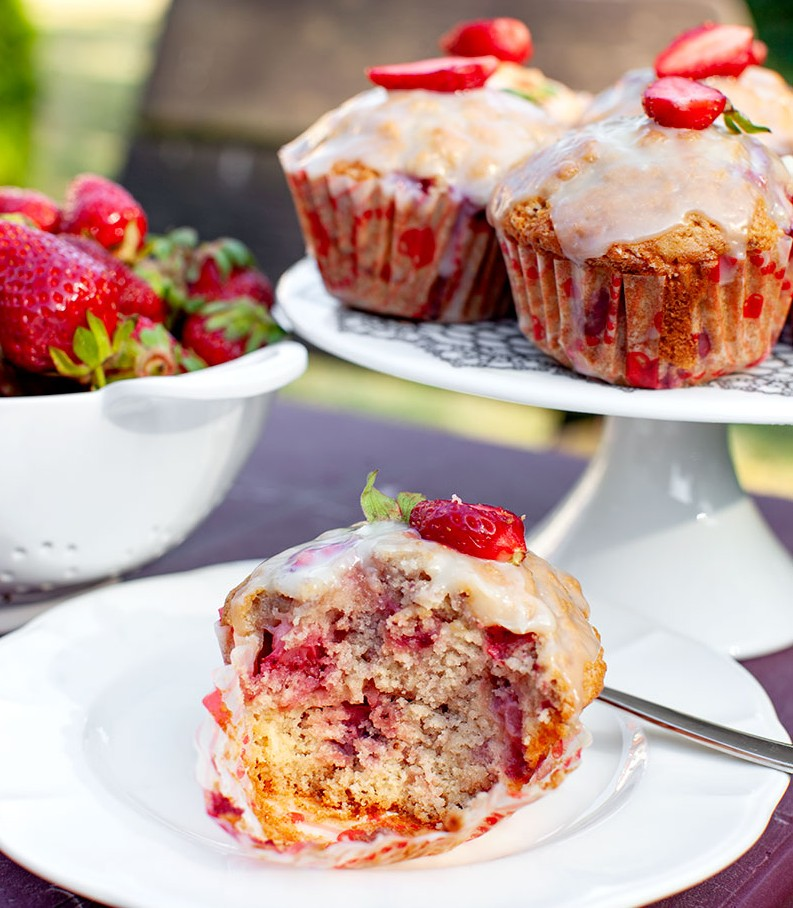
\includegraphics[width=0.4\textwidth]{muffiny_z_truskawkami.jpg}
    \end{wrapfigure}
    \begin{enumerate}
        \item 250 g truskawek
        \item 100 g roztopionego masła lub oleju roślinnego
        \item 125 ml mleka
        \item 2 jajka
        \item 250 g mąki pszennej
        \item 2 łyżeczki proszku do pieczenia
        \item 170 g cukru
    \end{enumerate}

    \paragraph{Przygotowanie:}
    \begin{enumerate}
        \item Truskawki opłukać, osuszyć i pokroić na kawałki. Piekarnik nagrzać
            do $180\celsius$. Formę na muffiny wyłożyć 12 papilotkami.
        \item Do miski wlać roztopione masło lub olej roślinny, dodać mleko,
            jajka i wymieszać np. rózgą.
        \item W drugiej misce wymieszać mąkę razem z proszkiem do pieczenia i
            cukrem.
        \item Wlać składniki z pierwszej miski i delikatnie wymieszać łyżką
            (tylko do czasu gdy nie będzie widać surowej mąki, nie można mieszać
            zbyt długo).  Pod koniec dodać truskawki i delikatnie wymieszać.
        \item Nałożyć równe porcje ciasta do papilotek i wstawić do nagrzanego
            piekarnika. Piec przez ok. 25 minut.
        \item Po przestudzeniu można polać polewą: roztopić czekoladę i
            wymieszać z jogurtem. Udekorować plasterkami truskawek i miętą.
    \end{enumerate}
    \newpage


    \subsection{Ciasto marchewkowe}
    \bigskip
    \paragraph{Składniki:}
    \begin{wrapfigure}[1]{r}{0.4\textwidth}
        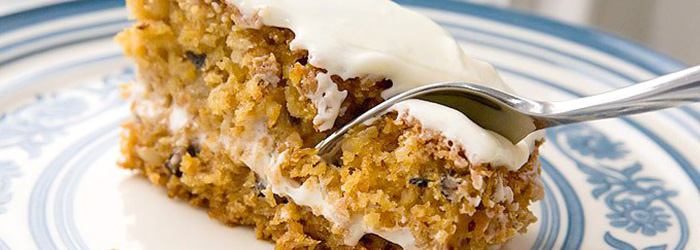
\includegraphics[width=0.4\textwidth]{ciasto_marchewkowe.jpg}
    \end{wrapfigure}
    \begin{enumerate}
        \item Ciasto:
            \begin{enumerate}
                \item 2 jajka
                \item 200 g drobnego cukru lub cukru pudru
                \item 150 ml oleju roślinnego
                \item 200 g drobno startej marchewki
                \item 50 g posiekanych orzechów włoskich lub pekan + do dekoracji
                \item 75 g drobno pokrojonego ananasa (świeżego lub z puszki) lub jabłka
                \item 50 g wiórków kokosowych
                \item 200 g mąki
                \item \sfrac{1}{2} łyżeczki proszku do pieczenia
                \item po 1 łyżeczce sody i cynamonu
                \item szczypta soli
            \end{enumerate}
        \item Polewa:
            \begin{enumerate}
                \item 125 g kremowego serka np. Twój Smak, Philadelphia
                \item 50 g masła (miękkiego)
                \item 100 g cukru pudru (lub mniej)
            \end{enumerate}
    \end{enumerate}

    \paragraph{Przygotowanie:}
    \begin{enumerate}
        \item Ciasto:
            \begin{enumerate}
                \item Jajka ocieplić w temperaturze pokojowej. Ubić je do
                    podwojenia objętości. Dodać cukier i dalej ubijać aż masa
                    będzie gładka i puszysta. Wciąż ubijając na wysokich
                    obrotach, dolewać ciągłym, cieniutkim strumieniem olej.
                \item Dodać marchewkę, ananasa, orzechy, wiórki kokosowe i
                    delikatnie wymieszać. Piekarnik nagrzać do 150 stopni C.
                \item Do osobnej miski przesiać mąkę, dodać proszek do
                    pieczenia, sodę, cynamon i sól, wymieszać. Przesypać do
                    miski z marchewką i delikatnie połączyć wszystkie składniki.
                \item Ciasto wyłożyć do formy o średnicy 24 cm wyłożonej
                    papierem do pieczenia. Piec przez 1 godzinę lub do suchego
                    patyczka.
            \end{enumerate}
        \item Polewa:
            \begin{enumerate}
                \item Ubić serek razem z miękkim masłem i cukrem pudrem. Włożyć na kilkanaście minut do lodówki.
                \item Dobrze wystudzone ciasto przekroić poziomo na 2 części.
                    Spód posmarować \sfrac{1}{3} ilości polewy.
                \item Przykryć drugą częścią ciasta i rozsmarować resztę polewy. Udekorować orzechami.
            \end{enumerate}
    \end{enumerate}
    \newpage

%    \subsection{Naleśniki}
%    \bigskip
%    \paragraph{Składniki:}
%    \begin{wrapfigure}[1]{r}{0.4\textwidth}
%        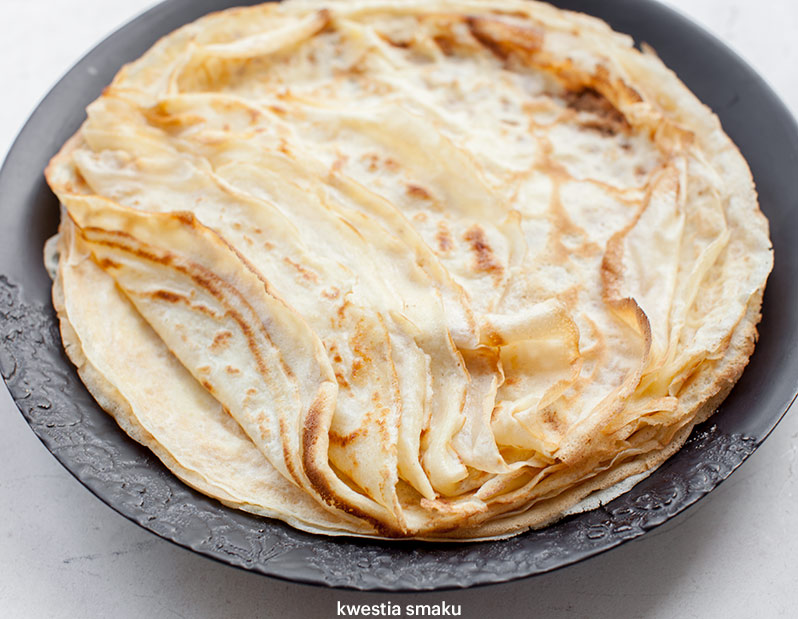
\includegraphics[width=0.4\textwidth]{nalesniki.jpg}
%    \end{wrapfigure}
%    \begin{enumerate}
%    \end{enumerate}
%
%    \paragraph{Przygotowanie:}
%    \begin{enumerate}
%    \end{enumerate}
%    \newpage

\end{document}

%    \subsection{Naleśniki}
%    \bigskip
%    \paragraph{Składniki:}
%    \begin{wrapfigure}[1]{r}{0.4\textwidth}
%        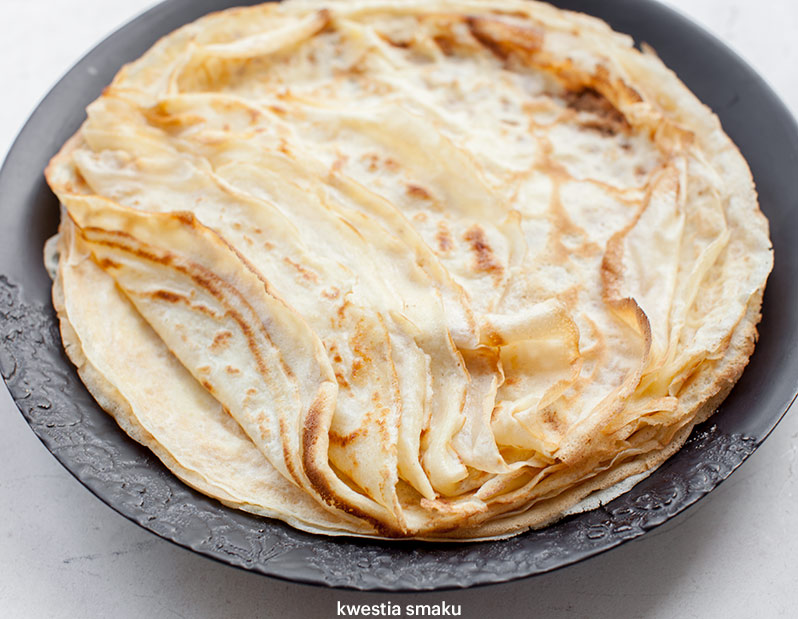
\includegraphics[width=0.4\textwidth]{nalesniki.jpg}
%    \end{wrapfigure}
%    \begin{enumerate}
%    \end{enumerate}
%
%    \paragraph{Przygotowanie:}
%    \begin{enumerate}
%    \end{enumerate}
%    \newpage
